% This presentation is based on a Beamer theme from Seth Brown, distributed
% under the following license:
%
% ----------------------------------------------------------------------------
% This program can be redistributed and/or modified under the terms
% of the GNU Public License, version 3.
%
% Seth Brown, Ph.D.
% sethbrown@drbunsen.org

\documentclass[t]{beamer}

\usepackage{hyperref} % urls
\usepackage{graphicx} % graphics
\usepackage[utf8x]{inputenc}
\usepackage{fancyvrb}
\usepackage{tcolorbox}

% suppress navigation bar
\beamertemplatenavigationsymbolsempty

\mode<presentation>
{
  \usetheme{codeplay}
  \setbeamercovered{transparent}
  \setbeamertemplate{itemize item}[circle]
  \setbeamertemplate{itemize subitem}{\tiny\raise1.5pt\hbox{\donotcoloroutermaths$\blacktriangleright$}}
  \setbeamertemplate{section in toc shaded}[default][100]
  \setbeamertemplate{subsection in toc shaded}[default][100]

\setbeamertemplate{subsection in toc}{%
\leavevmode\leftskip=4.00ex%
  \llap{\raisebox{0.15ex}{\textcolor{structure}{\small$\bullet$}}\kern1ex}%
  \inserttocsubsection\par%
}
}

% set fonts
\usepackage{fontspec}
\setsansfont{Calibri}
\setmonofont{Consolas}
\setbeamerfont{frametitle}{size=\LARGE,series=\bfseries}

% color definitions
\usepackage{color}
\definecolor{uiwhite}{RGB}{255, 255, 255}
\definecolor{uidarkgray}{RGB}{24,24,25}
\definecolor{uigray}{RGB}{51,51,51}
\definecolor{uilightgray}{RGB}{123,123,123}
\definecolor{uicyan}{RGB}{0,255,255}
\definecolor{uipink}{RGB}{255,153,255}
\definecolor{uipalegreen}{RGB}{153,255,153}
\hypersetup{colorlinks,urlcolor=uicyan,linkcolor=uiwhite}

% title slide definition
\title{Building an LLVM Backend}
\subtitle{LLVM 2014 tutorial}
\author{Fraser Cormack \\ Pierre-André Saulais}
\institute{Codeplay Software \\ @codeplaysoft}

\date{\today}

% Code box formatting
\fvset{fontsize=\scriptsize,tabsize=4}
\tcbset{colback=uigray,colframe=uilightgray,colupper=uiwhite,
        left=1pt,right=1pt,top=1pt,bottom=1pt,arc=0pt,
        toprule=1pt,bottomrule=1pt,leftrule=1pt,rightrule=1pt}

\newenvironment{codebox}
 {\VerbatimEnvironment
  \begin{tcolorbox}%
  \begin{Verbatim}}
 {\end{Verbatim}\end{tcolorbox}}

% Code caption that comes after the code box.
\newcommand{\codecaption}[2][-4.4ex]{%
  \vspace{#1}
  \hfill\mbox{\footnotesize{\textcolor{uicyan}{#2}}\hspace{0.5em}}
  \vspace*{2ex}}

\newcommand{\sourcebox}[3][firstline=1]{%
  \begin{tcolorbox}\VerbatimInput[#1]{#2}\end{tcolorbox}
  \codecaption{#3}}

\newcommand{\examplebox}[2][firstline=1]{\sourcebox[#1]{examples/#2}{#2}}

\newcommand{\codeempha}[1]{\textcolor{uipink}{#1}}
\newcommand{\codeemphb}[1]{\textcolor{uicyan}{#1}}
\newcommand{\codeemphc}[1]{\textcolor{uipalegreen}{#1}}

% FIXME: vfill doesn't work here!
\newcommand{\pipelinemap}[2]{\vspace{#2} #1}

% Create a slide for a part.
\newcommand{\talkpart}[2]{%
\section{Part #1: #2}

\begin{frame}[c]{Part #1}

\vspace{1cm}
\centerline{\LARGE{#2}}

\end{frame}}

% Create a slide for a part section.
\newcommand{\talksection}[1]{%
\subsection{#1}
\begin{frame}{\insertsectionhead}
\vspace{2ex}
\begin{NoHyper}
\tableofcontents[sectionstyle=hide,subsectionstyle=show/shaded/hide]
\end{NoHyper}
\end{frame}}

%%%%%%%%%%%%%%%%%%%%%%%%%%%%%%%%%%%%%%%%%%%%%%%%%%%%%%%%%%%%%%%%%%%%%%%%%%%%%%%%

\begin{document}

\setbeamertemplate{background}
{
\includegraphics[width=\paperwidth,height=\paperheight]{dark_background_title.png}}
\setbeamertemplate{footline}[default]

\begin{frame}
  \vspace{4ex}
  \titlepage
\end{frame}

%%%%%%%%%%%%%%%%%%%%%%%%%%%%%%%%%%%%%%%%%%%%%%%%%%%%%%%%%%%%%%%%%%%%%%%%%%%%%%%%

% Set the background for the rest of the slides.
%\setbeamertemplate{background}
% {
\includegraphics[width=\paperwidth,height=\paperheight]{dark_background.png}}
\setbeamertemplate{background}{}
\setbeamertemplate{footline}[codeplaytheme]

\section*{Introduction}

\begin{frame}{Introduction}

\begin{itemize}
    \item LLVM backend crash course, for beginners
    \begin{itemize}
        \item How-tos and tips
        \item Solution to common problems
    \end{itemize}  
    \item Example target created for this tutorial
    \begin{itemize}
        \item Can be used to see how LLVM works
        \item Can be used as a skeleton to bootstrap new target
    \end{itemize}
\end{itemize}

\end{frame}

%%%%%%%%%%%%%%%%%%%%%%%%%%%%%%%%%%%%%%%%%%%%%%%%%%%%%%%%%%%%%%%%%%%%%%%%%%%%%%%%

\begin{frame}{Overview}
\tableofcontents
\end{frame}

%%%%%%%%%%%%%%%%%%%%%%%%%%%%%%%%%%%%%%%%%%%%%%%%%%%%%%%%%%%%%%%%%%%%%%%%%%%%%%%%

\talkpart{1}{Background}
%%%%%%%%%%%%%%%%%%%%%%%%%%%%%%%%%%%%%%%%%%%%%%%%%%%%%%%%%%%%%%%%%%%%%%%%%%%%%%%%

\begin{frame}{What you need to start}

\begin{itemize}
    \item Know a little bit about LLVM IR: \\ \url{llvm.org/docs/LangRef.html}
    \item xdot.py to visualize graphs when debugging: \\ \url{github.com/jrfonseca/xdot.py}
    \item Check out and build our LLVM repo from GitHub: \\ \url{github.com/frasercrmck/llvm-leg}
    \item This informative and well-presented talk!
\end{itemize}

\end{frame}

%%%%%%%%%%%%%%%%%%%%%%%%%%%%%%%%%%%%%%%%%%%%%%%%%%%%%%%%%%%%%%%%%%%%%%%%%%%%%%%%

\begin{frame}{Example target: LEG}

\begin{itemize}
    \item Simple, RISC-like architecture
    \begin{itemize}
        \item Very small subset of ARM
    \end{itemize}
    \item 12 integer registers (32-bit)
    \begin{itemize}
        \item r0, r1, ..., r9, sp (stack pointer), lr (return address)
    \end{itemize}
    \item Instructions:
    \begin{itemize}
        \item 32-bit arithmetic (add, subtract, multiply, mad)
        \item 32-bit register move, 16-bit constant moves
        \item load, store, branch, branch and link
    \end{itemize}
\end{itemize}

\end{frame}

%%%%%%%%%%%%%%%%%%%%%%%%%%%%%%%%%%%%%%%%%%%%%%%%%%%%%%%%%%%%%%%%%%%%%%%%%%%%%%%%

\begin{frame}[fragile]{Calling convention for LEG}

\begin{itemize}
    \item How values are passed to/from a function
    \item Arguments in r0 (1st), r1 (2nd), …, r3 (4th)
    \begin{itemize}
        \item Further arguments passed on the stack
    \end{itemize}
    \item Return value in r0
\end{itemize}

\begin{codebox}
int foo(int a, int b) {
    int result = a + b;   // r0 + r1
    return result;        // r0
}
\end{codebox}
\codecaption{ex1.c}

\begin{codebox}
.foo:
    add r0, r0, r1
    b lr
\end{codebox}
\codecaption{ex1.s}

\end{frame}

%%%%%%%%%%%%%%%%%%%%%%%%%%%%%%%%%%%%%%%%%%%%%%%%%%%%%%%%%%%%%%%%%%%%%%%%%%%%%%%%

\begin{frame}{The big picture}

\begin{itemize}
    \item Pipeline structure of the backend:
    \begin{itemize}
        \item IR → SelectionDAG → MachineDAG  → MachineInstr → MCInst
    \end{itemize}
    \item Transforms your program many times
    \begin{itemize}
        \item Same program, few different representations
        \item Different instruction namespaces
        \item Check it out (IR and MI only):
        \begin{itemize}
            \item \texttt{llc foo.ll -print-after-all 2>\&1 > foo.log}
        \end{itemize}
    \end{itemize}
\end{itemize}

\end{frame}

%%%%%%%%%%%%%%%%%%%%%%%%%%%%%%%%%%%%%%%%%%%%%%%%%%%%%%%%%%%%%%%%%%%%%%%%%%%%%%%%

\begin{frame}[fragile]{A look at an IR module}

\begin{itemize}
    \item High-level, linear representation
    \item Typed values, no registers
    \item Target-agnostic
    \begin{itemize}
        \item Exceptions: data layout, triple, intrinsics
    \end{itemize}
\end{itemize}

\begin{codebox}[commandchars=\\\[\]]
target datalayout = "e-m:e-p:32:32-i1:8:32-i8:8:32-i16:16:32-i64:32-f64-..."
target triple = "leg"

define i32 @foo(i32 %a, i32 %b) {
    \codeempha[%c = add i32 %a, %b]
    ret i32 %c
}
\end{codebox}
\codecaption{ex1b.ll}

\end{frame}

%%%%%%%%%%%%%%%%%%%%%%%%%%%%%%%%%%%%%%%%%%%%%%%%%%%%%%%%%%%%%%%%%%%%%%%%%%%%%%%%

\begin{frame}{A look at a SelectionDAG graph}

\begin{minipage}[t]{0.50\linewidth}
    \begin{itemize}
        \item Graph representation
        \item Operations as nodes
        \begin{itemize}
            \item Mostly target-agnostic
            \item LEGISD (ISD) namespace
        \end{itemize}
        \item Dependencies as edges
        \begin{itemize}
            \item Data
            \item \codeemphb{Order ("chain")}
            \item \codeempha{Scheduling ("glue")}
        \end{itemize}
        \item Typed values
    \end{itemize}
\end{minipage}
\begin{minipage}[t]{0.49\linewidth}
    \begin{figure}
        \vspace{-2.2ex}
        
\includegraphics[width = 1.0\textwidth]{examples/ex1b/ex1b-pre-isel.pdf}
    \end{figure}
\end{minipage}

\end{frame}

%%%%%%%%%%%%%%%%%%%%%%%%%%%%%%%%%%%%%%%%%%%%%%%%%%%%%%%%%%%%%%%%%%%%%%%%%%%%%%%%

\begin{frame}{A look at a MachineDAG graph}

\begin{minipage}[t]{0.50\linewidth}
    \begin{itemize}
        \item Very similar to SelectionDAG
        \item Instructions as nodes
        \begin{itemize}
            \item Result of instruction selection
            \item LEG namespace
        \end{itemize}
        \item Similar dependencies
        \item Similar types
    \end{itemize}
\end{minipage}
\begin{minipage}[t]{0.49\linewidth}
    \begin{figure}
        \vspace{-2.2ex}
        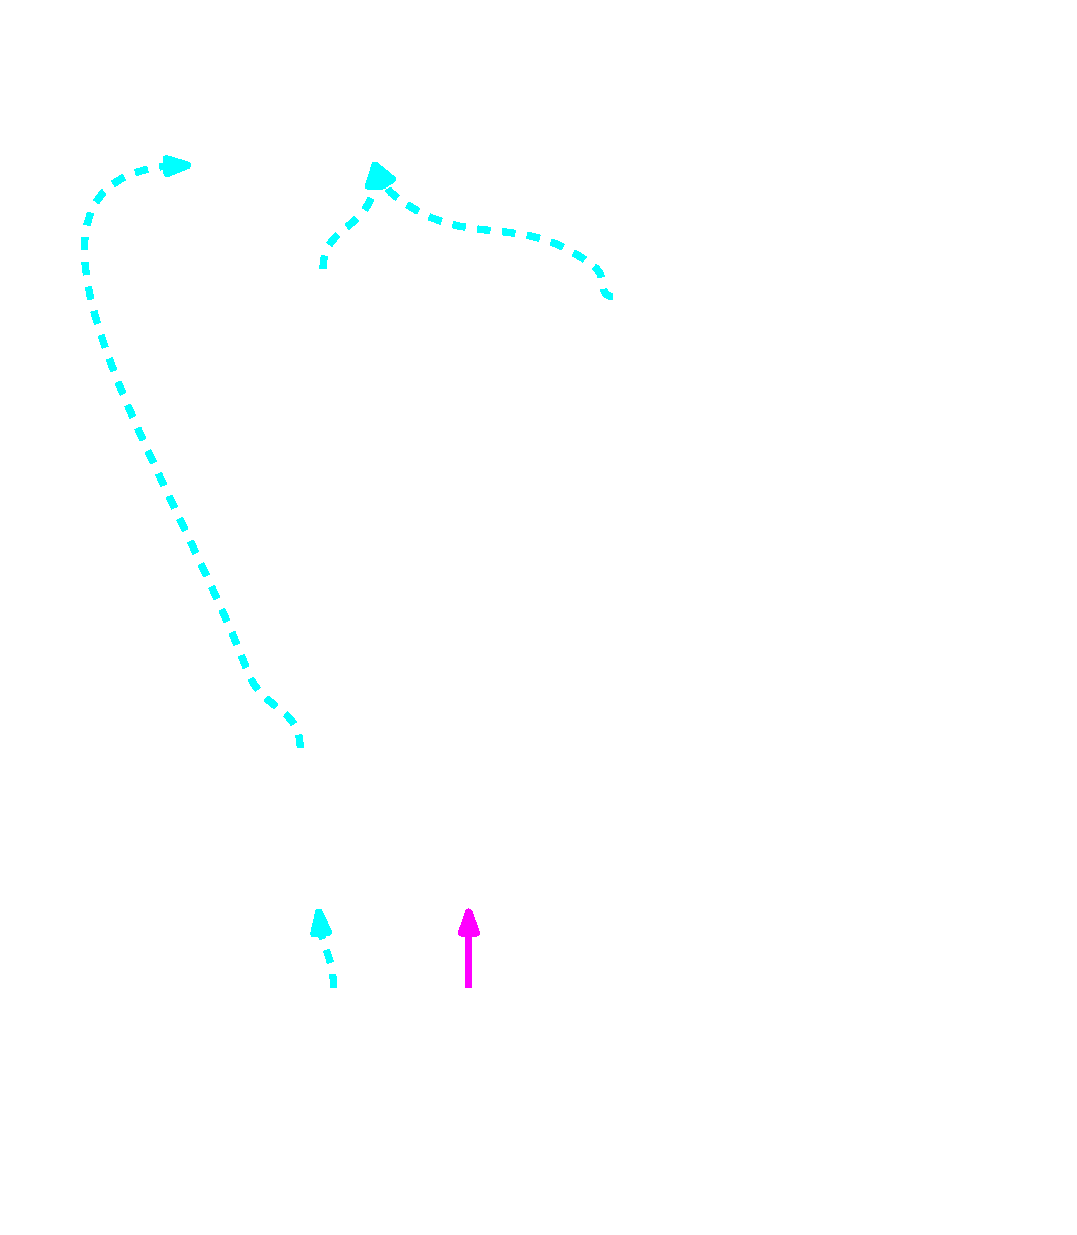
\includegraphics[width = 1.00\textwidth]{examples/ex1b/ex1b-post-isel.pdf}
    \end{figure}
\end{minipage}

\end{frame}

%%%%%%%%%%%%%%%%%%%%%%%%%%%%%%%%%%%%%%%%%%%%%%%%%%%%%%%%%%%%%%%%%%%%%%%%%%%%%%%%

\begin{frame}{Before and after ISel}

\begin{minipage}[t]{0.50\linewidth}
    \begin{figure}
        
\includegraphics[width = 1.00\textwidth]{examples/ex1b/ex1b-pre-isel.pdf}
    \end{figure}
\end{minipage}
\begin{minipage}[t]{0.49\linewidth}
    \begin{figure}
        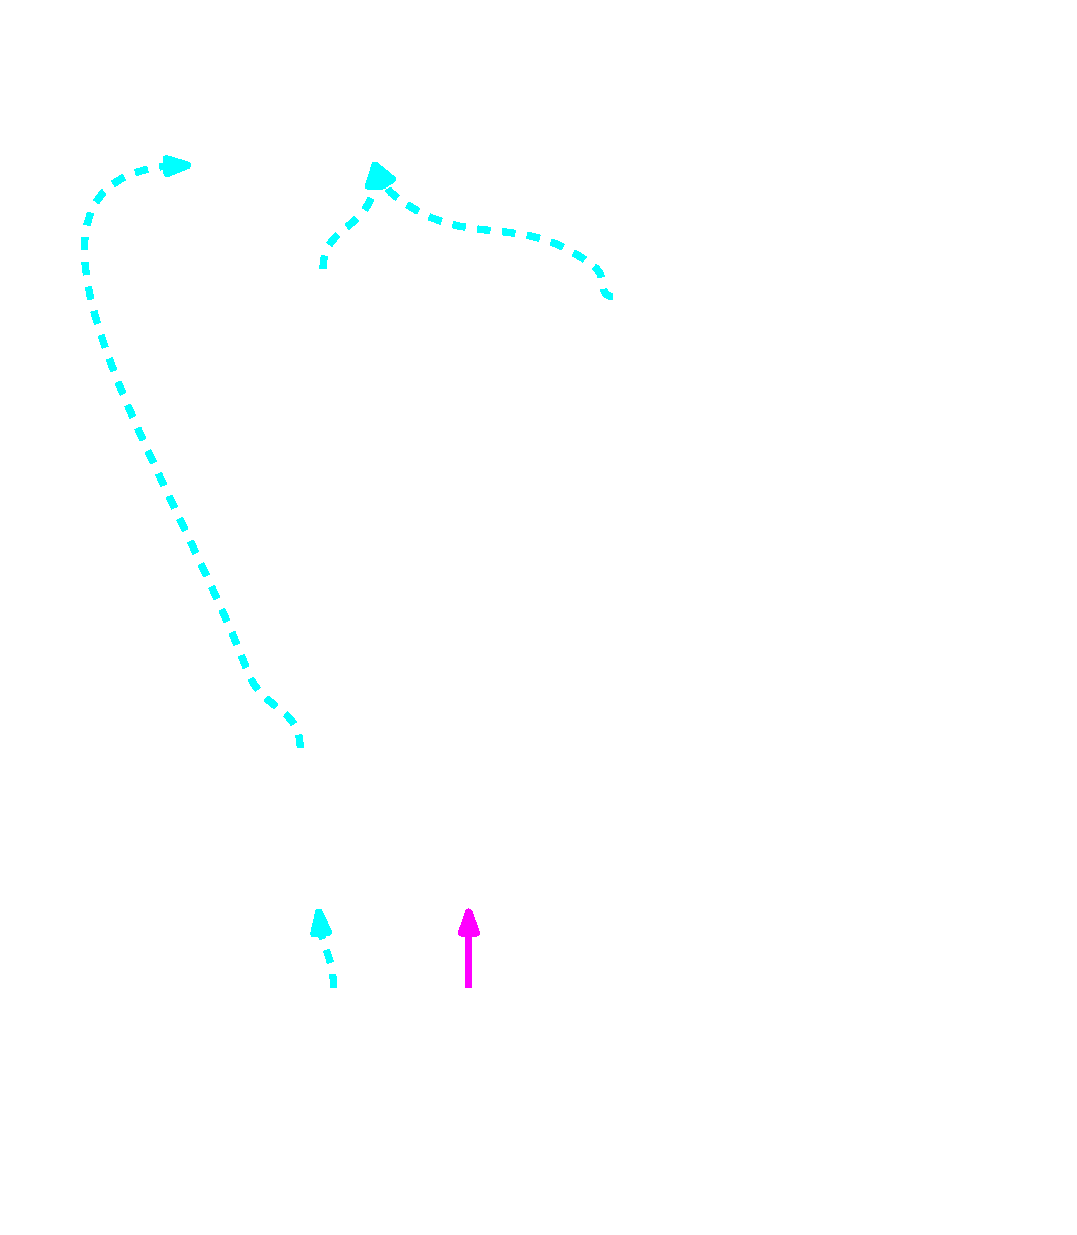
\includegraphics[width = 1.00\textwidth]{examples/ex1b/ex1b-post-isel.pdf}
    \end{figure}
\end{minipage}

\end{frame}

%%%%%%%%%%%%%%%%%%%%%%%%%%%%%%%%%%%%%%%%%%%%%%%%%%%%%%%%%%%%%%%%%%%%%%%%%%%%%%%%

\begin{frame}{A look at a MachineInstr block}

\begin{itemize}
    \item Untyped, uses register classes instead
    \item Target-specific instructions (LEG namespace)
    \begin{itemize}
        \item Few exceptions (TargetOpcode namespace)
    \end{itemize}
\end{itemize}

\examplebox{ex1/ex1-mi.txt}

\end{frame}


\talkpart{2}{Creating your own target}
%%%%%%%%%%%%%%%%%%%%%%%%%%%%%%%%%%%%%%%%%%%%%%%%%%%%%%%%%%%%%%%%%%%%%%%%%%%%%%%%

\begin{frame}{Bits of your ISA you need to describe}

\begin{itemize}
    \item Target machine
    \begin{itemize}
        \item Registers, register classes
        \item Calling conventions
    \end{itemize}
    \item Instruction set
    \begin{itemize}
        \item Operands and patterns
        \item Assembly printing and/or instruction encoding
        \item Schedule (not part of this talk)
    \end{itemize}
    \item ...
\end{itemize}

\end{frame}

%%%%%%%%%%%%%%%%%%%%%%%%%%%%%%%%%%%%%%%%%%%%%%%%%%%%%%%%%%%%%%%%%%%%%%%%%%%%%%%%

\begin{frame}{TableGen}

\begin{itemize}
    \item C++-style syntax
    \item Different set of backends
    \begin{itemize}
        \item RegisterInfo, InstrInfo, AsmWriter, ...
    \end{itemize}
    \item TableGen backends generate .inc files
    \begin{itemize}
        \item Included by your C++ files
    \end{itemize}
    \item More information:
    \begin{itemize}
        \item \url{llvm.org/docs/TableGen/index.html}
        \item \url{llvm.org/docs/TableGen/BackEnds.html}
    \end{itemize}
\end{itemize}

\end{frame}

%%%%%%%%%%%%%%%%%%%%%%%%%%%%%%%%%%%%%%%%%%%%%%%%%%%%%%%%%%%%%%%%%%%%%%%%%%%%%%%%

\begin{frame}[fragile]{Describing registers with TableGen}

\begin{itemize}
    \item TableGen provides the 'Register' class
    \begin{itemize}
        \item Can use the 'HWEncoding' field for encodings
    \end{itemize}
    \item Referenced as “LEG::R0” in C++
\end{itemize}

\begin{codebox}
class LEGReg<bits<16> Enc, string n> : Register<n> {
  Let HWEncoding = Enc;
  let Namespace = "LEG";
}

def R0 : LEGReg< 0, "r0" >;
...
def SP : LEGReg< 10, "sp" >;
\end{codebox}
\codecaption{LEGRegisterInfo.td}

\end{frame}

%%%%%%%%%%%%%%%%%%%%%%%%%%%%%%%%%%%%%%%%%%%%%%%%%%%%%%%%%%%%%%%%%%%%%%%%%%%%%%%%

\begin{frame}[fragile]{Describing registers with TableGen}

\begin{itemize}
    \item Can automate trivial definitions
\end{itemize}

\begin{codebox}
foreach i = 0-9 in {
  def R#i : R<i, "r"#i>;
}
\end{codebox}
\codecaption{LEGRegisterInfo.td}

\begin{itemize}
    \item Group registers into register classes
\end{itemize}

\begin{codebox}
def GRRegs : RegisterClass<"LEG", [i32], 32,
  (add SP, (sequence "R%i", 0, 9))>;
\end{codebox}
\codecaption{LEGRegisterInfo.td}

\end{frame}

%%%%%%%%%%%%%%%%%%%%%%%%%%%%%%%%%%%%%%%%%%%%%%%%%%%%%%%%%%%%%%%%%%%%%%%%%%%%%%%%

\begin{frame}[fragile]{Calling convention lowering: TableGen}

\begin{codebox}
def CC_LEG : CallingConv<[
    // Promote i8/i16 arguments to i32
    CCIfType<[i8, i16], CCPromoteToType<i32>>,

    // The first 4 arguments are passed in registers
    CCIfType<[i32], CCAssignToReg<[R0, R1, R2, R3]>>,

    // Fall-back, and use the stack
    CCIfType<[i32], CCAssignToStack<4, 4>>
  ]>;
\end{codebox}
\codecaption{LEGCallingConv.td}

\begin{itemize}
    \item Generates functions used in ISelLowering via function pointers.
\end{itemize}

\end{frame}

%%%%%%%%%%%%%%%%%%%%%%%%%%%%%%%%%%%%%%%%%%%%%%%%%%%%%%%%%%%%%%%%%%%%%%%%%%%%%%%%

\begin{frame}[fragile]{Calling convention lowering: The big picture}

\begin{columns}[t]
\column{.5\textwidth}
    \begin{codebox}[commandchars=\\\[\]]
define i32 @foo(i32 \codeempha[%a], i32 \codeemphb[%b]) {
    \codeemphc[%c] = add nsw i32 \codeempha[%a], \codeemphb[%b]
    ret i32 \codeemphc[%c]
}
    \end{codebox}
    \codecaption{ex1b.ll}

    Two target hooks:
    \begin{itemize}
            \item LowerFormalArguments()
            \item LowerReturn()
    \end{itemize}
\column{.5\textwidth}
    % FIXME Add 'a', 'b', 'c' circles
    \begin{block}{}
        \vspace{-5ex}
        
\includegraphics[width = 1.0\textwidth]{examples/ex1b/ex1b-pre-isel.pdf}
    \end{block}
\end{columns}    

\end{frame}

%%%%%%%%%%%%%%%%%%%%%%%%%%%%%%%%%%%%%%%%%%%%%%%%%%%%%%%%%%%%%%%%%%%%%%%%%%%%%%%%

\begin{frame}[fragile]{Calling convention lowering: The big picture}

\begin{columns}[t]
\column{.5\textwidth}
    LowerFormalArguments()
    \begin{itemize}
        \item Lowers incoming arguments into the DAG
    \end{itemize}

    LowerReturn()
    \begin{itemize}
        \item Lowers outgoing return values into the DAG
    \end{itemize}
    
\column{.5\textwidth}
    % FIXME Add 'a', 'b', 'c' circles and arrows from Lower*() to white circles
    \begin{block}{}
        \vspace{-5ex}
        
\includegraphics[width = 1.0\textwidth]{examples/ex1b/ex1b-pre-isel.pdf}
    \end{block}
\end{columns}    

\end{frame}

%%%%%%%%%%%%%%%%%%%%%%%%%%%%%%%%%%%%%%%%%%%%%%%%%%%%%%%%%%%%%%%%%%%%%%%%%%%%%%%%

\begin{frame}[fragile]{Calling convention lowering: LowerFormalArguments()}

\begin{itemize}
    \item Assigns locations to arguments, according to the TableGen-defined calling convention
    \item Creates DAG nodes for each location:
    \begin{itemize}
        \item Registers: CopyFromReg nodes
        \item Stack: frame indices and stack loads
    \end{itemize}
\end{itemize}

\begin{codebox}[commandchars=\\\[\]]
// LEGTargetLowering::LowerFormalArguments()
SmallVector<CCValAssign, 16> ArgLocs;
CCState CCInfo(CallConv, isVarArg, DAG.getMachineFunction(),
               getTargetMachine(), ArgLocs,
               *DAG.getContext());
CCInfo.AnalyzeFormalArguments(Ins, \codeempha[CC_LEG]);
...
\end{codebox}
\codecaption{LEGISelLowering.cpp}

\end{frame}

%%%%%%%%%%%%%%%%%%%%%%%%%%%%%%%%%%%%%%%%%%%%%%%%%%%%%%%%%%%%%%%%%%%%%%%%%%%%%%%%

\begin{frame}{Calling convention lowering: LowerReturn()}

\begin{itemize}
    \item Similar to \texttt{LowerFormalArguments()}, but the other way around
    \item Define another, \texttt{RetCC\_LEG}, TableGen calling convention
    \item Call 'AnalyzeReturn()' with it
    \item Walk the return value locations and issue DAG nodes
    \item Return \texttt{LEGISD::RET} instruction
\end{itemize}

\end{frame}

%%%%%%%%%%%%%%%%%%%%%%%%%%%%%%%%%%%%%%%%%%%%%%%%%%%%%%%%%%%%%%%%%%%%%%%%%%%%%%%%

\begin{frame}{Calling convention lowering: LowerCall()}

\begin{itemize}
    \item Hybrid of \texttt{LowerFormalArguments()} and \texttt{LowerReturn()}
    \item Not explicitly covered here
\end{itemize}

\end{frame}

%%%%%%%%%%%%%%%%%%%%%%%%%%%%%%%%%%%%%%%%%%%%%%%%%%%%%%%%%%%%%%%%%%%%%%%%%%%%%%%%

\begin{frame}{Describing instructions: Overview}

\begin{itemize}
    \item Let's start with a simple instruction: \texttt{ADDrr}
    \item Define it in lib/Target/LEG/LEGInstrInfo.td
    \item What we need to specify:
    \begin{itemize}
        \item Operands
        \item Assembly string
        \item Instruction pattern
    \end{itemize}
\end{itemize}

\end{frame}

%%%%%%%%%%%%%%%%%%%%%%%%%%%%%%%%%%%%%%%%%%%%%%%%%%%%%%%%%%%%%%%%%%%%%%%%%%%%%%%%

\begin{frame}[fragile]{Describing instructions: Operands}

\begin{itemize}
    \item List of definitions or outputs ('outs')
    \item List of uses or inputs ('ins')
    \item Operand class:
    \begin{itemize}
        \item Register class (e.g. GRRegs)
        \item Immediate (e.g. i32imm)
        \item More complex operands (e.g. reg + imm for load/store)
    \end{itemize}
\end{itemize}

\begin{codebox}[commandchars=\\\{\}]
def ADDrr : InstLEG<\codeempha{(outs GRRegs:$dst)},
                    \codeempha{(ins GRRegs:$src1, GRRegs:$src2)},
                    "add $dst, $src1, $src2",
                    [(set i32:$dst, (add i32:$src1, i32:$src2))]>;
\end{codebox}
\codecaption[-10.2ex]{LEGInstrInfo.td}

\end{frame}

%%%%%%%%%%%%%%%%%%%%%%%%%%%%%%%%%%%%%%%%%%%%%%%%%%%%%%%%%%%%%%%%%%%%%%%%%%%%%%%%

\begin{frame}[fragile]{Describing instructions: Selection Patterns}

\begin{itemize}
    \item Matches nodes in the SelectionDAG
    \begin{itemize}
        \item Nodes get turned into MachineInstrs during ISel
        \item If pattern is omitted, selection needs to be done in C++
    \end{itemize}
    \item Syntax:
    \begin{itemize}
        \item One pair of parenthesis defines one node
        \item Nodes have DAG operands, with 'MVT' type (e.g. i32)
        \item Map DAG operands to MI operands
    \end{itemize}
\end{itemize}

\begin{codebox}[commandchars=\\\{\}]
def ADDrr : InstLEG<(outs GRRegs:$dst),
                    (ins GRRegs:$src1, GRRegs:$src2),
                    "add $dst, $src1, $src2",
                    \codeempha{[(set i32:$dst, (add i32:$src1, i32:$src2))]}>;
\end{codebox}
\codecaption[-10.2ex]{LEGInstrInfo.td}

\end{frame}

%%%%%%%%%%%%%%%%%%%%%%%%%%%%%%%%%%%%%%%%%%%%%%%%%%%%%%%%%%%%%%%%%%%%%%%%%%%%%%%%

\begin{frame}[fragile]{Describing instructions: Result}

\begin{itemize}
    \item This is what we get after defining the pattern:
    \item Assembly was generated by the instruction printer
    \begin{itemize}
        \item More on this later
    \end{itemize}
\end{itemize}

% FIXME move to file
\begin{codebox}
# BB#0:                                 # %entry
	add r0, r0, r1
\end{codebox}
\codecaption{ex1.s}

\begin{codebox}[commandchars=\\\{\}]
def ADDrr : InstLEG<(outs GRRegs:$dst),
                    (ins GRRegs:$src1, GRRegs:$src2),
                    \codeempha{"add $dst, $src1, $src2"},
                    [(set i32:$dst, (add i32:$src1, i32:$src2))]>;
\end{codebox}
\codecaption[-10.2ex]{LEGInstrInfo.td}

\end{frame}

%%%%%%%%%%%%%%%%%%%%%%%%%%%%%%%%%%%%%%%%%%%%%%%%%%%%%%%%%%%%%%%%%%%%%%%%%%%%%%%%

\begin{frame}[fragile]{Constants}

\begin{itemize}
    \item Compiling this IR produces the following error:
\end{itemize}

\begin{codebox}
%2 = add nsw i32 %1, 2
\end{codebox}
\codecaption{ex2.ll}

\begin{codebox}
LLVM ERROR: Cannot select: 0x29d4350: i32 = Constant<2> [ID=2]
In function: main
\end{codebox}

\begin{itemize}
    \item Specify how to generate ('materialize') constants
    \item For example, with a 'move' instruction
    \begin{itemize}
        \item E.g. MOVW on ARM for 16-bit constants
    \end{itemize}
\end{itemize}

\end{frame}

%%%%%%%%%%%%%%%%%%%%%%%%%%%%%%%%%%%%%%%%%%%%%%%%%%%%%%%%%%%%%%%%%%%%%%%%%%%%%%%%

\begin{frame}[fragile]{Constants}

\begin{itemize}
    \item Let's define this move instruction:
\end{itemize}

\begin{codebox}
def MOVWi16 : InstLEG<(outs GRRegs:$dst),
                      (ins i32imm:$src),
                      "movw $dst, $src",
                      [(set i32:$dst, i32imm:$src)]> {
  let isMoveImm = 1;
}
\end{codebox}
\codecaption{LEGInstrInfo.td}

\begin{itemize}
    \item The previous example translates to:
\end{itemize}

\examplebox[firstline=7,lastline=8,gobble=1]{ex2/ex2-ADDrr-MOVW.s}

\end{frame}

%%%%%%%%%%%%%%%%%%%%%%%%%%%%%%%%%%%%%%%%%%%%%%%%%%%%%%%%%%%%%%%%%%%%%%%%%%%%%%%%

\begin{frame}[fragile]{Constants}

What if instructions take immediates?

\begin{codebox}[commandchars=\\¬|]
def \codeempha¬LEGimm8| : Operand<i32>, ImmLeaf<i32, [{
  return Imm >= 0 && Imm < 256;
}]>;

def ADDri : InstLEG<(outs GRRegs:$dst),
                    (ins GRRegs:$src1, \codeempha¬i32imm|:$src2),
                    "add $dst, $src1, $src2",
                    [(set i32:$dst, (add i32:$src1, 
                                     \codeempha¬LEGimm8|:$src2))]>;
\end{codebox}
\codecaption{LEGInstrInfo.td}

Output:

\examplebox[firstline=7,lastline=7,gobble=1]{ex2/ex2-ADDri.s}

\end{frame}

%%%%%%%%%%%%%%%%%%%%%%%%%%%%%%%%%%%%%%%%%%%%%%%%%%%%%%%%%%%%%%%%%%%%%%%%%%%%%%%%

\begin{frame}[fragile]{Matching multiple DAG nodes}

\begin{itemize}
    \item DAG nodes can be nested inside selection patterns
    \begin{itemize}
        \item The output of one node is the input of another
    \end{itemize}
    \item Allows operations to be combined
    \begin{itemize}
        \item Reduces the number of generated instructions
        \item Possibly improves performance or power consumption
    \end{itemize}
    \item Example: multiply and add instruction (ex3.ll)
\end{itemize}

\begin{codebox}[commandchars=\\\{\}]
def MLA : InstLEG<(outs GRRegs:$dst),
                  (ins GRRegs:$src1, GRRegs:$src2, GRRegs:$src3),
                  "mla $dst, $src1, $src2, $src3",
                  [(set i32:$dst,
                   \codeempha{(add \codeemphb{(mul i32:$src1, i32:$src2)}, i32:$src3))}]>;
\end{codebox}
\codecaption[-12.2ex]{LEGInstrInfo.td}

\end{frame}

%%%%%%%%%%%%%%%%%%%%%%%%%%%%%%%%%%%%%%%%%%%%%%%%%%%%%%%%%%%%%%%%%%%%%%%%%%%%%%%%

\begin{frame}[fragile]{Matching multiple DAG nodes}

% FIXME center image, add dotted line circles, arrows
% FIXME also add text "With MLA pattern" and assembly output, "Without" etc
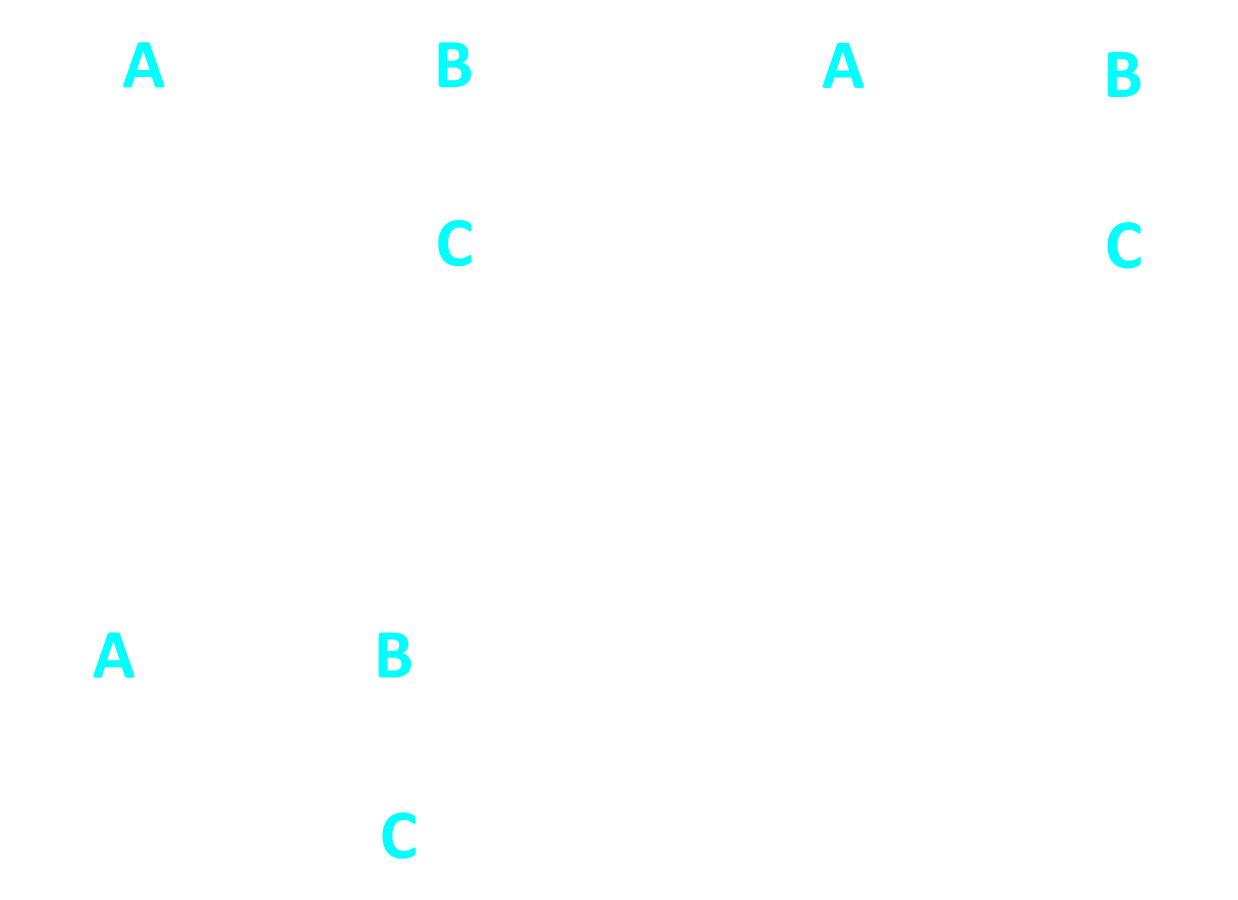
\includegraphics[width = 0.80\textwidth]{examples/ex3/ex3-selection1.png}

\end{frame}

%%%%%%%%%%%%%%%%%%%%%%%%%%%%%%%%%%%%%%%%%%%%%%%%%%%%%%%%%%%%%%%%%%%%%%%%%%%%%%%%

\begin{frame}{Frame lowering}

\begin{itemize}
    \item Hooks invoked when values are stored on the stack
    \begin{itemize}
        \item In debug builds (-O0), but not only
    \end{itemize}
    \item Adjust the stack at the beginning ('prologue') and end ('epilogue') of functions
    \begin{itemize}
        \item LEGFrameLowering::emitPrologue()
        \item LEGFrameLowering::emitEpilogue()
    \end{itemize}
    \item Usually by increasing or decreasing the stack pointer
    \item May need to align the stack pointer too
\end{itemize}

\end{frame}

%%%%%%%%%%%%%%%%%%%%%%%%%%%%%%%%%%%%%%%%%%%%%%%%%%%%%%%%%%%%%%%%%%%%%%%%%%%%%%%%

\begin{frame}{Frame lowering}

\begin{itemize}
    \item Example that uses the stack:
\end{itemize}

\examplebox[firstline=7,lastline=10]{ex4/ex4.ll}

\begin{itemize}
    \item Output when compiled with -O2:
\end{itemize}

\examplebox[firstline=7,lastline=11]{ex4/ex4-O2.s}

\end{frame}

%%%%%%%%%%%%%%%%%%%%%%%%%%%%%%%%%%%%%%%%%%%%%%%%%%%%%%%%%%%%%%%%%%%%%%%%%%%%%%%%

\begin{frame}[fragile]{Frame lowering}

\begin{itemize}
    \item When compiling with  -O0, hooks need to be defined
    \item Emit load/store instructions with frame indices
    \item Minimal implementation:
\end{itemize}

\begin{codebox}
// LEGInstrInfo::storeRegToStackSlot()
BuildMI(MBB, I, I->getDebugLoc(), get(LEG::STR))
  .addReg(SrcReg, getKillRegState(KillSrc))
  .addFrameIndex(FrameIndex).addImm(0);

// LEGInstrInfo::loadRegFromStackSlot()
BuildMI(MBB, I, I->getDebugLoc(), get(LEG::LDR), DestReg)
  .addFrameIndex(FrameIndex).addImm(0);

// LEGInstrInfo::copyPhysReg()
BuildMI(MBB, I, I->getDebugLoc(), get(LEG::MOVrr), DestReg)
  .addReg(SrcReg, getKillRegState(KillSrc));

\end{codebox}
\codecaption{LEGFrameLowering.cpp}

\end{frame}

%%%%%%%%%%%%%%%%%%%%%%%%%%%%%%%%%%%%%%%%%%%%%%%%%%%%%%%%%%%%%%%%%%%%%%%%%%%%%%%%

\begin{frame}{Instruction printer}

\begin{itemize}
    \item New classes:
    \begin{itemize}
        \item LEGAsmPrinter
        \item LEGMCInstLower
        \item An MCAsmStreamer (usually stock)
        \item LEGInstPrinter
    \end{itemize}
    \item LEGAsmPrinter works as a gateway to the streamers
    \item This stages works with MCInsts, lowered from MachineInstrs by LEGMCInstLower
\end{itemize}

\end{frame}

%%%%%%%%%%%%%%%%%%%%%%%%%%%%%%%%%%%%%%%%%%%%%%%%%%%%%%%%%%%%%%%%%%%%%%%%%%%%%%%%

\begin{frame}[fragile]{Instruction printer}

\begin{itemize}
    \item TableGen provides the 'AsmString' field:
\end{itemize}

\begin{codebox}
class InstLEG<... , string asmstr> : Instruction {
  let AsmString = asmstr;
  ...
}
\end{codebox}
\codecaption{LEGInstrFormats.t}

\begin{codebox}[commandchars=\\\[\]]
def ADDrr : InstLEG<(outs GRRegs:$dst),
                    (ins GRRegs:$src1, GRRegs:$src2),
                    \codeempha["add $dst, $src1, $src2"]> {
  ...
}
\end{codebox}
\codecaption{LEGInstrInfo.td}

\begin{itemize}
    \item \texttt{LEGInstPrinter::printOperand} will be called on each operand.
\end{itemize}

\end{frame}

%%%%%%%%%%%%%%%%%%%%%%%%%%%%%%%%%%%%%%%%%%%%%%%%%%%%%%%%%%%%%%%%%%%%%%%%%%%%%%%%

\begin{frame}[fragile]{Instruction printer}

\begin{itemize}
    \item \texttt{LEGInstPrinter::printOperand} is given the stream to print to.
\end{itemize}

\begin{codebox}
void LEGInstPrinter::printOperand(const MCInst *MI, unsigned No,
                                  raw_ostream &O) {
  const MCOperand &Op = MI->getOperand(No);
  if (Op.isReg()) {
    // TableGen generates this function for us from   
    // LEGRegisterInfo.td
    O << getRegisterName(Op.getReg());
    return;
  }
  if (Op.isImm()) {
    O << '#' << Op.getImm();
    return;
  }
  /* ... */
}
\end{codebox}
\codecaption{LEGInstPrinter.cpp}

\end{frame}

%%%%%%%%%%%%%%%%%%%%%%%%%%%%%%%%%%%%%%%%%%%%%%%%%%%%%%%%%%%%%%%%%%%%%%%%%%%%%%%%

\begin{frame}{Instruction printer}

\begin{itemize}
    \item That's it!
    \item Directives and labels handled for us
    \begin{itemize}
        \item Can emit target-specific syntax if we wish
    \end{itemize}
\end{itemize}

\examplebox[firstline=1,lastline=10]{ex1/ex1.s}

\end{frame}


\talkpart{3}{How-tos for specific tasks}
%%%%%%%%%%%%%%%%%%%%%%%%%%%%%%%%%%%%%%%%%%%%%%%%%%%%%%%%%%%%%%%%%%%%%%%%%%%%%%%%

\talksection{Instruction printing}

\begin{frame}{Instruction printer}

\begin{itemize}
    \item New classes:
    \begin{itemize}
        \item LEGAsmPrinter
        \item LEGMCInstLower
        \item An MCAsmStreamer (usually stock)
        \item LEGInstPrinter
    \end{itemize}
    \item LEGAsmPrinter works as a gateway to the streamers
    \item This stages works with MCInsts, lowered from MachineInstrs by LEGMCInstLower
\end{itemize}

\end{frame}

%%%%%%%%%%%%%%%%%%%%%%%%%%%%%%%%%%%%%%%%%%%%%%%%%%%%%%%%%%%%%%%%%%%%%%%%%%%%%%%%

\begin{frame}[fragile]{Instruction printer}

\begin{itemize}
    \item TableGen provides the 'AsmString' field:
\end{itemize}

\begin{codebox}
class InstLEG<... , string asmstr> : Instruction {
  let AsmString = asmstr;
  ...
}
\end{codebox}
\codecaption{LEGInstrFormats.t}

\begin{codebox}[commandchars=\\\[\]]
def ADDrr : InstLEG<(outs GRRegs:$dst),
                    (ins GRRegs:$src1, GRRegs:$src2),
                    \codeempha["add $dst, $src1, $src2"]> {
  ...
}
\end{codebox}
\codecaption{LEGInstrInfo.td}

\begin{itemize}
  \item \texttt{LEGInstPrinter::printOperand()} will be called on each operand.
\end{itemize}

\end{frame}

%%%%%%%%%%%%%%%%%%%%%%%%%%%%%%%%%%%%%%%%%%%%%%%%%%%%%%%%%%%%%%%%%%%%%%%%%%%%%%%%

\begin{frame}[fragile]{Instruction printer}

\begin{itemize}
  \item \texttt{LEGInstPrinter::printOperand()} prints the assembly string of a given operand...
\end{itemize}

\begin{codebox}
void LEGInstPrinter::printOperand(const MCInst *MI, unsigned No,
                                  raw_ostream &O) {
  const MCOperand &Op = MI->getOperand(No);
  if (Op.isReg()) {
    // TableGen generates this function for us from   
    // LEGRegisterInfo.td
    O << getRegisterName(Op.getReg());
    return;
  }
  if (Op.isImm()) {
    O << '#' << Op.getImm();
    return;
  }
  /* ... */
}
\end{codebox}
\codecaption{LEGInstPrinter.cpp}

\begin{itemize}
  \item ...and is given the stream to print it to
\end{itemize}

\end{frame}

%%%%%%%%%%%%%%%%%%%%%%%%%%%%%%%%%%%%%%%%%%%%%%%%%%%%%%%%%%%%%%%%%%%%%%%%%%%%%%%%

\begin{frame}{Instruction printer}

\begin{itemize}
    \item That's it!
    \item Directives and labels handled for us
    \begin{itemize}
        \item Can emit target-specific syntax if we wish
    \end{itemize}
\end{itemize}

\examplebox[firstline=1,lastline=10]{ex1/ex1.s}

\end{frame}

%%%%%%%%%%%%%%%%%%%%%%%%%%%%%%%%%%%%%%%%%%%%%%%%%%%%%%%%%%%%%%%%%%%%%%%%%%%%%%%%

\talksection{Instruction encoding}

\begin{frame}{Instruction encoding}

\begin{itemize}
    \item A few new classes:
    \begin{itemize}
        \item An MCObjectStreamer (again, stock)
        \item LEGMCCodeEmitter
        \item LEGObjectWriter
        \item LEGAsmBackend
    \end{itemize}
    \item You will also need your LEGAsmPrinter
\end{itemize}

\end{frame}

%%%%%%%%%%%%%%%%%%%%%%%%%%%%%%%%%%%%%%%%%%%%%%%%%%%%%%%%%%%%%%%%%%%%%%%%%%%%%%%%

\begin{frame}[fragile]{Instruction encoding}

Example encoding:

\vspace{1ex}

\begin{tabular}{|c|c|c|c|c|c|c|c|}
\hline 
31...28 & 27...25 & 24...21 & 20 & 19...16 & 15...12 & 11...4 & 3...0\tabularnewline
\hline 
1110 & 000 & opcode & 0 & src1 & dst & 00000000 & src2\tabularnewline
\hline 
\end{tabular}

\vspace{2ex}

How can we achieve this?

\vspace{1ex}

\begin{codebox}[commandchars=\\\{\}]
def ADDrr : InstLEG<(outs GRRegs:$dst),
                    (ins GRRegs:$src1, GRRegs:$src2),
                    "add $dst, $src1, $src2",
                    [(set i32:$dst, (add i32:$src1, i32:$src2))]>;
\end{codebox}
\codecaption[-10.2ex]{LEGInstrInfo.td}

\end{frame}

%%%%%%%%%%%%%%%%%%%%%%%%%%%%%%%%%%%%%%%%%%%%%%%%%%%%%%%%%%%%%%%%%%%%%%%%%%%%%%%%

\begin{frame}[fragile]{Instruction encoding}

\begin{itemize}
    \item TableGen recognises the 'Inst' field:
\end{itemize}

\begin{codebox}
class InstLEG< ... > : Instruction {
  field bits<32> Inst;
  ...
}
\end{codebox}
\codecaption{LEGInstrFormats.td}

\begin{itemize}
    \item Used to define the binary encoding of each instruction in TableGen:
\end{itemize}

\begin{codebox}
def ADDrr : InstLEG< ... > {
  let Inst{31-25} = 0b110000;
  let Inst{24-21} = 0b1100;      // Opcode
  let Inst{20}    = 0b0;
  let Inst{11-4}  = 0b00000000;
}
\end{codebox}
\codecaption{LEGInstrInfo.td}

\end{frame}

%%%%%%%%%%%%%%%%%%%%%%%%%%%%%%%%%%%%%%%%%%%%%%%%%%%%%%%%%%%%%%%%%%%%%%%%%%%%%%%%

\begin{frame}[fragile]{Instruction encoding}

\begin{itemize}
    \item For operand-based encoding, need bit fields with the same names as the operands:
\end{itemize}

\begin{codebox}[commandchars=\\\[\]]
def ADDrr : InstLEG<(outs GRRegs:\codeemphc[$dst]),
                    (ins GRRegs:\codeempha[$src1], GRRegs:\codeemphb[$src2]) ... > {
  bits<4> \codeempha[src1]; bits<4> \codeemphb[src2]; bits<4> \codeemphc[dst];
  let Inst{31-25} = 0b110000;
  let Inst{24-21} = 0b1100;      // Opcode
  let Inst{20}    = 0b0;
  let Inst{19-16} = \codeempha[src1];        // Operand 1
  let Inst{15-12} = \codeemphc[dst];         // Destination
  let Inst{11-4}  = 0b00000000;
  let Inst{3-0}   = \codeemphb[src2];        // Operand 2
\end{codebox}
\codecaption{LEGInstrInfo.td}

\begin{itemize}
    \item \texttt{LEGMCCodeEmitter::getMachineOpValue()} will be called on each operand
\end{itemize}

\end{frame}

%%%%%%%%%%%%%%%%%%%%%%%%%%%%%%%%%%%%%%%%%%%%%%%%%%%%%%%%%%%%%%%%%%%%%%%%%%%%%%%%

\begin{frame}[fragile]{Instruction encoding}

\begin{itemize}
  \item \texttt{LEGMCCodeEmitter::getMachineOpValue()} returns the binary encoding of a given operand...
\end{itemize}

\begin{codebox}
unsigned LEGMCCodeEmitter::
getMachineOpValue(const MCInst &MI, const MCOperand MO,
                  SmallVectorImpl<MCFixup> &Fixups,
                  const MCSubtargetInfo &STI) const {
  if (MO.isReg()) {
    return
      CTX.getRegisterInfo()->getEncodingValue(MO.getReg());
  } if (MO.isImm()) {
    return static_cast<unsigned>(MO.getImm());
  }
  /* ... */
}
\end{codebox}
\codecaption{LEGMCCodeEmitter.cpp}

\begin{itemize}
  \item ...which is placed, masked, and shifted into position by TableGen-erated code
\end{itemize}

\end{frame}

%%%%%%%%%%%%%%%%%%%%%%%%%%%%%%%%%%%%%%%%%%%%%%%%%%%%%%%%%%%%%%%%%%%%%%%%%%%%%%%%

\begin{frame}[fragile]{Relocations and fixups}

\begin{itemize}
    \item For values that need fixing up, record the relocation and return zero
    \item LLVM will keep track of the relocation for us and help us fix it up later
\end{itemize}

\begin{codebox}
unsigned LEGMCCodeEmitter::
getMachineOpValue(const MCInst &MI, const MCOperand MO,
                  SmallVectorImpl<MCFixup> &Fixups,
                  const MCSubtargetInfo &STI) const {
  /* ... */

  assert(MO.isExpr()); // MO must be an expression
  
  const MCExpr *Expr = MO.getExpr();
  const MCExpr::ExprKind Kind = Expr->getFixupKind();

  Fixups.push_back(MCFixup::Create(0, Expr, Kind));
  return 0;
}
\end{codebox}
\codecaption{LEGMCCodeEmitter.cpp}

\end{frame}

%%%%%%%%%%%%%%%%%%%%%%%%%%%%%%%%%%%%%%%%%%%%%%%%%%%%%%%%%%%%%%%%%%%%%%%%%%%%%%%%

\begin{frame}[fragile]{Relocations and fixups}

\begin{itemize}
    \item Defining a target-specific fixup:
\end{itemize}

\begin{codebox}
enum Fixups {
  fixup_leg_mov_hi16_pcrel = FirstTargetFixupKind,
  fixup_leg_mov_lo16_pcrel,
  
  LastTargetFixupKind,
  NumTargetFixupKinds = LastTargetFixupKind - FirstTargetFixupKind
};
\end{codebox}
\codecaption{LEGFixups.h}

\begin{codebox}
const MCFixupKindInfo& getFixupKindInfo(MCFixupKind K) const {
  const static MCFixupKindInfo I[LEG::NumTargetFixupKinds] = {
    // Name          Offset Size Flags
    { "fixup_leg_mov_hi16_pcrel", 0,  32, MCFixupKindInfo::FKF_IsPCRel },
    { "fixup_leg_mov_lo16_pcrel", 0,  32, MCFixupKindInfo::FKF_IsPCRel },
  };
  /* ... */
  return I[K - FirstTargetFixupKind];
}
\end{codebox}
\codecaption{LEGAsmBackend.cpp}

\end{frame}

%%%%%%%%%%%%%%%%%%%%%%%%%%%%%%%%%%%%%%%%%%%%%%%%%%%%%%%%%%%%%%%%%%%%%%%%%%%%%%%%

\begin{frame}{Relocations and fixups}

\begin{itemize}
    \item We must then implement some hooks
    \item These are called at the end once the section layouts have been finalized
    \item \texttt{LEGAsmBackend::processFixupValue()}
    \begin{itemize}
        \item Adjusts the fixup value, e.g., splitting the value across non-contiguous fields
    \end{itemize}
    \item \texttt{LEGAsmBackend::applyFixup()}
    \begin{itemize}
        \item Patches the fixed-up value into the binary stream
    \end{itemize}
\end{itemize}

\end{frame}

%%%%%%%%%%%%%%%%%%%%%%%%%%%%%%%%%%%%%%%%%%%%%%%%%%%%%%%%%%%%%%%%%%%%%%%%%%%%%%%%

\talksection{Selection DAG manipulation}

\begin{frame}[fragile]{Custom SelectionDAG nodes}

\begin{itemize}
    \item To represent target-specific operations in the DAG
    \begin{itemize}
        \item Example: 32-bit immediate move
    \end{itemize}
    \item How?
    \begin{itemize}
        \item Add a value in the \texttt{LEGISD} enum
        \item Update \texttt{LEGTargetLowering::getTargetNodeName()}
        \item Add TableGen node definitions
        \begin{itemize}
            \item Type definition: number of inputs, outputs, constraints
            \item Node definition: tablegen name, opcode, type
        \end{itemize}
    \end{itemize}
    \item Custom nodes can be used in TableGen selection patterns
\end{itemize}

\begin{codebox}
def MoveImm32Ty : SDTypeProfile<1, 1, [
  SDTCisSameAs<0, 1>, SDTCisInt<0>
]>;

def movei32 : SDNode<"LEGISD::MOVi32", MoveImm32Ty>;
\end{codebox}
\codecaption{LEGOperators.td}

\end{frame}

%%%%%%%%%%%%%%%%%%%%%%%%%%%%%%%%%%%%%%%%%%%%%%%%%%%%%%%%%%%%%%%%%%%%%%%%%%%%%%%%

\begin{frame}[fragile]{Custom DAG lowering}

\begin{itemize}
    \item To handle DAG nodes in a special way
    \begin{itemize}
        \item Replaces an existing node with one or more other DAG nodes
        \item Matches nodes by opcode (e.g. \texttt{ISD::Constant})
        \item Matches nodes by type (e.g. \texttt{i32})
    \end{itemize}
    \item How?
    \begin{itemize}
        \item Call \texttt{setOperationAction(\emph{nodeOpcode}, type, Custom)}
        \item Create a function to handle it (e.g. \texttt{LowerOPCODE})
        \item Update \texttt{LowerOperation} to call \texttt{LowerOPCODE}
    \end{itemize}
    \item This all hapens in \texttt{LEGTargetLowering} (\texttt{LEGISelLowering.cpp})
\end{itemize}

\end{frame}

%%%%%%%%%%%%%%%%%%%%%%%%%%%%%%%%%%%%%%%%%%%%%%%%%%%%%%%%%%%%%%%%%%%%%%%%%%%%%%%%

\begin{frame}[fragile]{Custom DAG lowering: \texttt{LowerOPCODE}}

\begin{itemize}
    \item \texttt{LowerOPCODE} takes a DAG node (\texttt{Op}) and returns a DAG node
    \item You can:
    \begin{itemize}
        \item Return a different node
        \item Return \texttt{Op} → no change
        \item Return \texttt{SDValue()} → node not supported (LLVM will expand it)
    \end{itemize}
    \item All of the above can be done conditionally (e.g. depending on \texttt{VT})
\end{itemize}

\begin{codebox}
SDValue LEGTargetLowering::LowerConstant(SDValue Op,
                                         SelectionDAG &DAG) const {
  EVT VT = Op.getValueType();
  ConstantSDNode *Val = cast<ConstantSDNode>(Op.getNode());
  SDValue TargetVal = DAG.getTargetConstant(Val->getZExtVaue(),
                                            MVT::i32);
  return DAG.getNode(LEGISD::MOVi32, VT, TargetVal);
}
\end{codebox}
\codecaption{LEGISelLowering.cpp}

\end{frame}

%%%%%%%%%%%%%%%%%%%%%%%%%%%%%%%%%%%%%%%%%%%%%%%%%%%%%%%%%%%%%%%%%%%%%%%%%%%%%%%%

\begin{frame}[fragile]{Creating SelectionDAG nodes}

\begin{itemize}
    \item Simply call \texttt{DAG.getNode()} with these arguments:
    \begin{itemize}
        \item Node opcode (e.g. \texttt{LEGISD::MOVi32}), type, operand(s)
    \end{itemize}
    \item Nodes are target-independent (\texttt{ISD}) or not (\texttt{LEGISD})
    \item Use \texttt{DAG.getMachineNode()} in LEGISelDAGToDAG
\end{itemize}

\begin{codebox}
SDValue LEGTargetLowering::LowerConstant(SDValue Op,
                                         SelectionDAG &DAG) const {
  EVT VT = Op.getValueType();
  ConstantSDNode *Val = cast<ConstantSDNode>(Op.getNode());
  SDValue TargetVal = DAG.getTargetConstant(Val->getZExtVaue(),
                                            MVT::i32);
  return DAG.getNode(LEGISD::MOVi32, VT, TargetVal);
}
\end{codebox}
\codecaption{LEGISelLowering.cpp}

\end{frame}

%%%%%%%%%%%%%%%%%%%%%%%%%%%%%%%%%%%%%%%%%%%%%%%%%%%%%%%%%%%%%%%%%%%%%%%%%%%%%%%%

\begin{frame}{Lowering to multiple instructions}

\begin{minipage}[t]{0.58\linewidth}
    \begin{itemize}
        \item Example: 32-bit immediate load
        \begin{itemize}
            \item MOVLO: loads 16-bit 'low' part
            \item MOVHI: loads 16-bit 'high' part
        \end{itemize}
        
        \item The two instructions must be ordered
        \begin{itemize}
            \item \texttt{MOVLO} clears the 'high' part
            \item \texttt{MOVHI, MOVLO} gives the wrong result
            \item Make \texttt{MOVHI} read the output of \texttt{MOVLO}
        \end{itemize}
        \item Example: \texttt{0x00010002}
    \end{itemize}
\end{minipage}
\begin{minipage}[t]{0.41\linewidth}
    \begin{figure}
        \vspace{-3.5ex}
        
\includegraphics[width = 1.00\textwidth]{examples/ex5/ex5-post-isel.pdf}
    \end{figure}
\end{minipage}

\end{frame}

%%%%%%%%%%%%%%%%%%%%%%%%%%%%%%%%%%%%%%%%%%%%%%%%%%%%%%%%%%%%%%%%%%%%%%%%%%%%%%%%

\begin{frame}[fragile]{Lowering to multiple instructions}

\begin{itemize}
    \item To define MOVHI, we need an extra operand ('\texttt{fakesrc}')
    \begin{itemize}
        \item Source and destination registers must be the same
        \item Use '\texttt{Constraints}' in Tablegen
    \end{itemize}
\end{itemize}

\begin{codebox}[commandchars=\\¬|]
def MOVHIi16 : InstLEG<(outs GRRegs:$dst),
                      (ins \codeempha¬GRRegs:$fakesrc|, i32imm:$src),
                      "movt $dst, $src",
                      [/* No pattern */]> {
  let Constraints = "$fakesrc = $dst";
}
\end{codebox}
\codecaption{LEGInstrInfo.td}

\end{frame}

%%%%%%%%%%%%%%%%%%%%%%%%%%%%%%%%%%%%%%%%%%%%%%%%%%%%%%%%%%%%%%%%%%%%%%%%%%%%%%%%

\begin{frame}{Lowering to multiple instructions}

\begin{itemize}
    \item Different ways to emit multiple instructions from one DAG node
    \begin{itemize}
        \item Using custom C++ instruction selection code
            \begin{itemize}
                \item Not covered here
            \end{itemize}
        \item Using a pseudo-instruction as a placeholder
    \end{itemize}
\end{itemize}

\end{frame}

%%%%%%%%%%%%%%%%%%%%%%%%%%%%%%%%%%%%%%%%%%%%%%%%%%%%%%%%%%%%%%%%%%%%%%%%%%%%%%%%

\begin{frame}[fragile]{Lowering to multiple instructions}

\begin{itemize}
    \item Using a pseudo instruction
    \begin{itemize}
        \item Behaves like a placeholder for 'real' machine instruction(s)
        \item Lowered by a target hook into these instruction instructions
        \item Can be selected from the custom DAG node we previously defined
    \end{itemize}
\end{itemize}

\begin{codebox}
def MOVi32 : InstLEG<(outs GRRegs:$dst), (ins i32imm:$src), "",
                     [(set i32:$dst, (movei32 i32imm:$src))]> {
  let isPseudo = 1;
}
\end{codebox}
\codecaption{LEGInstrInfo.td}

\end{frame}

%%%%%%%%%%%%%%%%%%%%%%%%%%%%%%%%%%%%%%%%%%%%%%%%%%%%%%%%%%%%%%%%%%%%%%%%%%%%%%%%

\begin{frame}[fragile]{Lowering to multiple instructions}

\begin{itemize}
    \item The pseudo is lowered by a target hook
\end{itemize}


\begin{codebox}
bool LEGInstrInfo::expandPostRAPseudo(MachineInstr *MI) {
  if (MI->getOpcode() != LEG::MOVi32)
    return false;
    
  DebugLoc DL = MI->getDebugLoc();
  MachineBasicBlock &MBB = *MI->getParent();
  unsigned Dst = MI->getOperand(0).getReg();
  unsigned Imm = MI->getOperand(1).getImm();
  unsigned Lo16 = Imm & 0xffff;
  unsigned Hi16 = (Imm >> 16) & 0xffff;

  BuildMI(MBB, MI, DL, get(LEG::MOVLOi16), Dst).addImm(Lo16);
  BuildMI(MBB, MI, DL, get(LEG::MOVHIi16), Dst).addReg(Dst).addImm(Hi16);
   
  MBB.erase(MI);
  
  return true;
}
\end{codebox}
\codecaption{LEGInstrInfo.cpp}

\end{frame}

%%%%%%%%%%%%%%%%%%%%%%%%%%%%%%%%%%%%%%%%%%%%%%%%%%%%%%%%%%%%%%%%%%%%%%%%%%%%%%%%

\begin{frame}{Lowering to multiple instructions}

Example IR:
\examplebox[firstline=6,lastline=9]{ex5/ex5.ll}

Resulting assembly:
\examplebox[firstline=7,lastline=11,gobble=1]{ex5/ex5.s}

\end{frame}


\talkpart{4}{Troubleshooting and resources}
\section{Part 4: Troubleshooting and tips}

\begin{frame}{Part 4}

Background

\end{frame}

%%%%%%%%%%%%%%%%%%%%%%%%%%%%%%%%%%%%%%%%%%%%%%%%%%%%%%%%%%%%%%%%%%%%%%%%%%%%%%%%

\begin{frame}{When something goes wrong}

\begin{itemize}
    \item Find which pass introduces the issue:
    \begin{itemize}
        \item \texttt{llc -print-after-all}
    \end{itemize}
    \item Find the LLVM source file and category for this pass:
    \begin{itemize}
        \item \texttt{\#define DEBUG\_TYPE "codegen-dce"}
    \end{itemize}
    \item Dump the log:
    \begin{itemize}
        \item \texttt{llc foo.ll -debug-only codegen-dce 2>\&1 > foo.log}
    \end{itemize}
    \item Compare (diff) the \texttt{-print-after-all} or \texttt{-debug-only} good and bad outputs to see where it goes wrong
\end{itemize}

\end{frame}

%%%%%%%%%%%%%%%%%%%%%%%%%%%%%%%%%%%%%%%%%%%%%%%%%%%%%%%%%%%%%%%%%%%%%%%%%%%%%%%%

\begin{frame}{Debugging LLVM}

\begin{itemize}
    \item MIs, BBs, functions, almost anything → call \texttt{X.dump()}
    \item DAGs, CFGs → call \texttt{X.viewGraph()} (pops up xdot)
    \item Or from the terminal: \texttt{llc foo.ll -view-isel-dags}
    \begin{itemize}
        \item Try -view-dag1-combine-dags, -view-legalize-dags, -view-sched-dags, etc.
    \end{itemize}
    \item To view graphs, make sure you build LLVM in debug mode!
    \begin{itemize}
        \item Turn on \texttt{LLVM\_ENABLE\_ASSERTIONS} (i.e. \texttt{NDEBUG} should not be defined)
    \end{itemize}
\end{itemize}

\end{frame}

%%%%%%%%%%%%%%%%%%%%%%%%%%%%%%%%%%%%%%%%%%%%%%%%%%%%%%%%%%%%%%%%%%%%%%%%%%%%%%%%

\begin{frame}{"Cannot select"}

\begin{itemize}
    \item When LLVM doesn't know how to map ('lower') a DAG node to an actual instruction
    \begin{itemize}
        \item Missing pattern in \texttt{LEGInstrInfo.td}?
        \item Without a pattern, lowering needs to be done in \texttt{LEGISelDAGToDag::Select()}
    \end{itemize}
    \item Check the graph!
\end{itemize}

\end{frame}

%%%%%%%%%%%%%%%%%%%%%%%%%%%%%%%%%%%%%%%%%%%%%%%%%%%%%%%%%%%%%%%%%%%%%%%%%%%%%%%%

\begin{frame}{The dog ate my homework}

\begin{itemize}
    \item Why did my code disappear?
    \begin{itemize}
        \item Missing chain/glue in the DAG
        \item Dead code elimination may have removed it
    \end{itemize}
    \item DCE does not touch instructions whose value is used by other instructions:
    \begin{itemize}
        \item Root your use/def chains using a MI that has side-effects
    \end{itemize}
    \item DCE does not touch instructions with side-effects:
    \begin{itemize}
        \item \texttt{mayLoad}, \texttt{mayStore}, \texttt{isTerminator}, \texttt{hasSideEffects}
    \end{itemize}
\end{itemize}

\end{frame}

%%%%%%%%%%%%%%%%%%%%%%%%%%%%%%%%%%%%%%%%%%%%%%%%%%%%%%%%%%%%%%%%%%%%%%%%%%%%%%%%

\begin{frame}{Useful in-tree resources}

\begin{itemize}
    \item include/llvm/Target/Target*.h
    \begin{itemize}
        \item Shows all target-specific hooks that can be overridden, with useful comments
    \end{itemize}
    \item include/llvm/Target/Target*.td
    \begin{itemize}
        \item Shows all TableGen fields you can use in your target files
    \end{itemize}
    \item include/llvm/CodeGen/ISDOpcodes.h
    \begin{itemize}
        \item Lists all SelectionDAG nodes and descriptions of what they mean
    \end{itemize}
\end{itemize}

\end{frame}

%%%%%%%%%%%%%%%%%%%%%%%%%%%%%%%%%%%%%%%%%%%%%%%%%%%%%%%%%%%%%%%%%%%%%%%%%%%%%%%%

\begin{frame}{You're not alone!}

\begin{itemize}
    \item "Writing an LLVM Backend" at \url{llvm.org/docs/WritingAnLLVMBackend.html}
    \item Other backends 
    \item TableGen backend documentation
    \item LLVM-Dev mailing lists
    \item Anton Korobeynikov's 2009 and 2012 "Building a backend in 24 hours" tutorials
\end{itemize}

\end{frame}


%%%%%%%%%%%%%%%%%%%%%%%%%%%%%%%%%%%%%%%%%%%%%%%%%%%%%%%%%%%%%%%%%%%%%%%%%%%%%%%%

\section*{Conclusion}

\begin{frame}{Summary}

\begin{itemize}
    \item Should be enough to create a very simple target!
    \item Many things were not covered in this talk:
    \begin{itemize}
        \item Using different types and legalization
        \item Scheduling
        \item Intrinsics
        \item ...
    \end{itemize}
    \item Introduced resources to go further
\end{itemize}

\end{frame}

%%%%%%%%%%%%%%%%%%%%%%%%%%%%%%%%%%%%%%%%%%%%%%%%%%%%%%%%%%%%%%%%%%%%%%%%%%%%%%%%

\begin{frame}{Thank you!}

\begin{itemize}
    \item Q\&A
    \item Happy to answer questions by email too:
    \begin{itemize}
        \item \url{fraser@codeplay.com}
        \item \url{pierre-andre@codeplay.com}
    \end{itemize}
    \item Check out our code from GitHub:
    \begin{itemize}
        \item \url{github.com/frasercrmck/llvm-leg}
    \end{itemize}
\end{itemize}

\end{frame}

%%%%%%%%%%%%%%%%%%%%%%%%%%%%%%%%%%%%%%%%%%%%%%%%%%%%%%%%%%%%%%%%%%%%%%%%%%%%%%%%

\end{document}
